\chapter{先行研究}
\section{深層学習}
一般に,機械学習で使用されるモデルは決定木,サポートベクターマシン(SVM),ニューラルネットワークなどが存在する.決定木は得られた予測に対して,どの説明変数が影響したのかの判断が容易であり,説明可能性が高いことで知られている.
一方で,ニューラルネットワークは,パーセプトロンを筆頭に,層の増加やネットワークの複雑化が図られてきた.黎明期においては,非線形な問題をとけるように知見が盛り込まれたSVMや,生物が持つ視覚野の知見から提案されたネオコグニトロンなどの画期的な手法が提案されてきた.その中でも,ネオコグニトロンに端を発する,畳み込みニューラルネットワーク(CNN)は,LeNet\cite{LeNet}により,誤差逆伝播法が導入され,2010年代以降には,AlexNet\cite{AlexNet},VGGNet\cite{VGGNet},ResNet\cite{ResNet},と急速に進化を遂げてきた.
このような深層化されたニューラルネットワークは興味深い性質や振る舞いを示す.しかし,そのような性質がどのような機序によって引き起こされるかについての完全な合意はとられていない.

\section{二重降下現象}
機械学習において,モデルの性能はモデルの複雑性(例えば,パラメータ数)と深い関係があり,モデルのパラメータ数が不足することによるアンダーフィッティング(Underfitting)\cite{underfitting}や,過剰なパラメータによるオーバーフィッティング(Overfitting)\cite{overfitting}などの現象が知られている.モデルの複雑性が増すにつれて,初めは性能が向上し(アンダーフィッティングを克服),その後過剰な複雑性により性能が低下するとされていた.これはU字型のカーブ,いわゆるバイアス-バリアンス トレードオフ\cite{Rajnarayan2010}として知られている.

ところが近年発見されたDouble Descent\cite{Belkin_2019}と呼ばれている現象は,モデルの複雑性がさらに増すと,性能が再び向上する.つまり,最初のU字型のカーブ(アンダーフィッティングからオーバーフィッティングへの移行)の後,さらに複雑性が増加すると,新たな性能向上のフェーズが現れるのである.過剰パラメータを持つディープニューラルネットワークが,理論的にはオーバーフィッティングを起こすべきなのに,実際には優れた汎化性能を示す場合がある\cite{ResNet,ViT}.

このDouble Descentは,Belkinら\cite{Belkin_2019}によって決定木や二層のニューラルネットワークで確認され,その後,Nakkiranら\cite{nakkiran2021deep}が,ディープニューラルネットワーク(DNN)においても観察されること,学習エポック数の増加に対してもDouble Descentが起こることを示した.さらに,パラメータの枝刈りによるスパース性の増加に対してもDouble Descentが起こることが報告されている\cite{He}.パラメータ数,学習エポック数,スパース性の増加に伴って観察されるDouble Descentは,それぞれ,Model-wise Double Descent,Epoch-wise Double Descent,Sparse Double Descent と呼ばれている\cite{nakkiran2021deep,He}.

\section{画像認識における形状・テクスチャ}
Geirhosらは,ImageNetで学習したCNNが,分類のために特に画像のテクスチャを重視することを示した~\cite{Geirhos}.彼らは,相反する形状とテクスチャ情報を持つ画像をCNNに入力し,出力が形状ベースのラベルとテクスチャベースのラベルのどちらに一致するかをチェックした.この結果に基づいて,CNNが認識において形状とテクスチャのどちらを優先するかを分析した.一方,Islamらは,ニューロンの潜在表現に基づくモデルにおいて,形状とテクスチャのどちらを重視するかを定量的に判断する方法を提案した~\cite{Islam}.この方法によって,CNNがどの特徴に偏重するのかを定量的に分析することができる.さらに,Geらは人間の視覚系のモデル化を試み,Human Vision System (HVS)を開発した.HVSは,画像分類時にどの特徴(形状,テクスチャ,色など)が最も重要な役割を果たすかを定量的に評価可能である\cite{Ge}.

\section{画像認識における二重降下現象と形状・テクスチャバイアスの関係}
\begin{figure}[t]
    \centering
    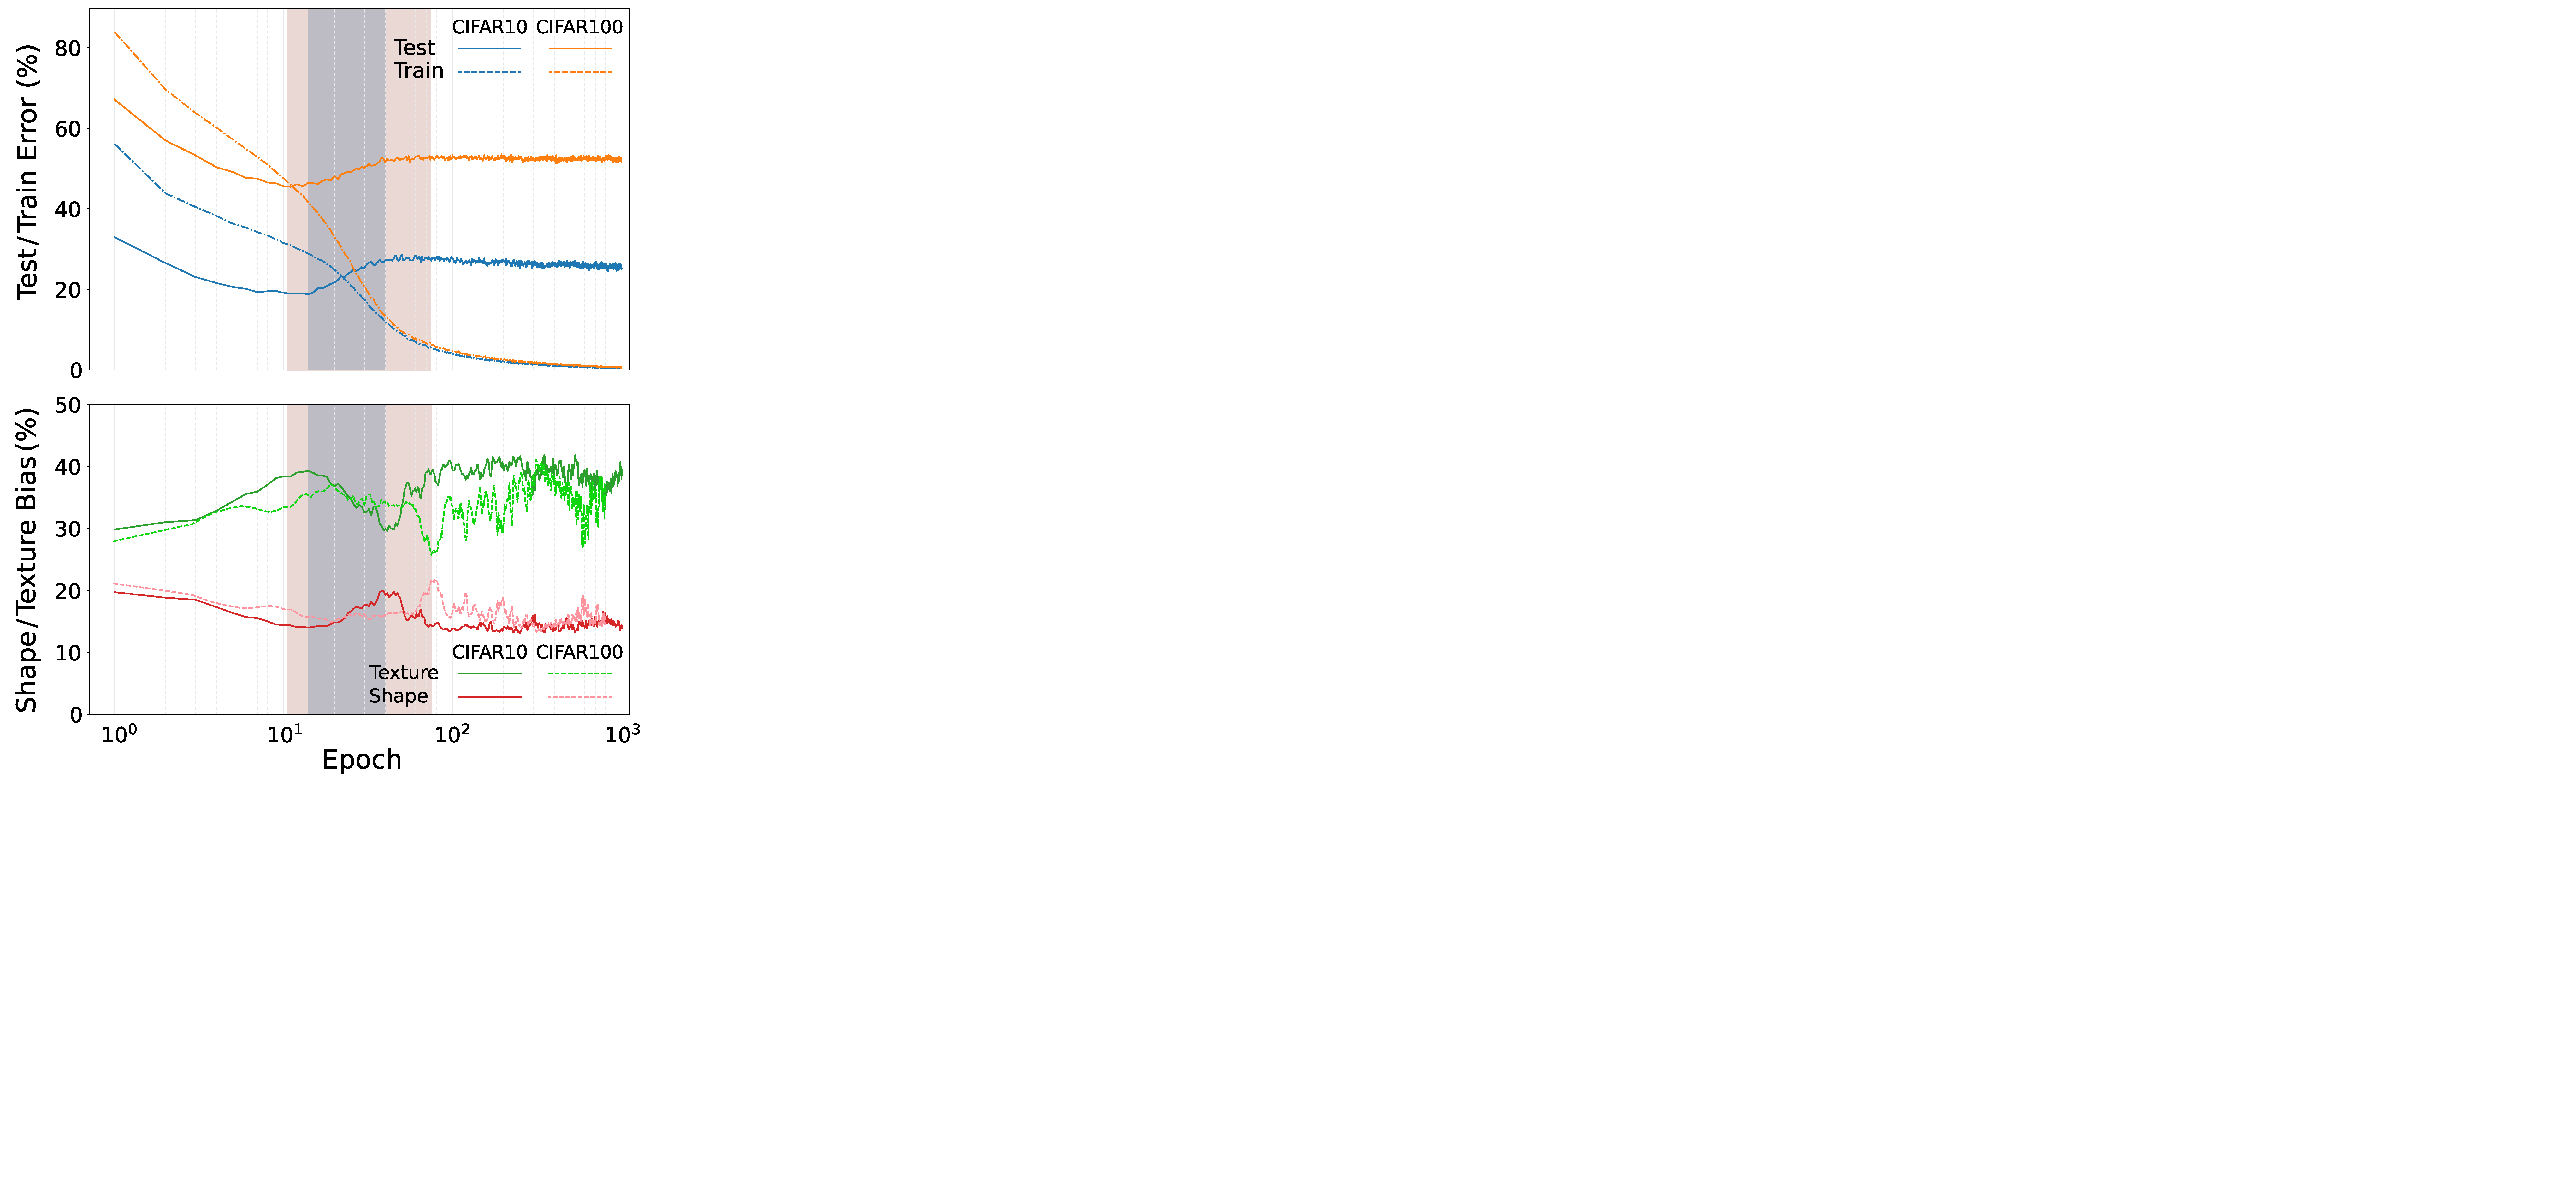
\includegraphics[width=\linewidth]{fig/iwaseICPR.pdf}
    \caption{ResNet18の学習過程におけるDDとSTBとの同期性}
    \label{fig:iwaseICPR}
\end{figure}
\UTF{9AD9}橋らの研究~\cite{DD_STB}は,画像認識タスクにおける二重降下現象と,CNNの形状バイアスおよびテクスチャバイアスの変化の関連性を示唆した.この研究では,二重降下現象と形状・テクスチャバイアスの変化のタイミングに相関が見られ,テスト誤り率が上昇から下降に転じるタイミングと,形状バイアスが増加し始めるタイミングが一致することが示された.
また,事前学習の有無による学習過程の違いも観測された.事前学習ありのモデルでは初期からテクスチャバイアスが高く,学習が進むと形状バイアスが増加する傾向が見られた.一方,事前学習なしのモデルでは学習初期は形状バイアスが高く,その後テクスチャバイアスが増加する傾向が確認された.

岩瀬らの研究~\cite{icpr2024iwase}では,さらに形状・テクスチャバイアスと二重降下現象に関する同期性を様々な角度から検証している.この研究では,CIFAR-10とResNet18の組み合わせ以外の条件下で同期性が確認されたほか,どの層が要因となり,同期性が起こっているのかが明らかとなった.
これらの知見は,画像認識モデルの学習ダイナミクスと二重降下現象の関係性に新たな洞察を提供している.
この同期性を図\ref{fig:iwaseICPR}に示す.
これまでの研究では,CNNの学習過程における形状とテクスチャという特徴の獲得と二重降下現象の関係について研究されてきた.そこで,本研究では形状とテクスチャではなく,色と数字という概念を設定し,2つの学習過程における概念獲得の過程の観測した.
\newpage